\section[最小二乘方程]{最小二乘方程\\The Equations of Least Squares}
本章提出了全球定位的基本数学。在大图片中,我们获得卫星到接收机的伪距测量值。有如此多的卫星,我们希望有更多测量值而不是最少的测量值去确定X,Y,Z,t(位置和时间)。但是这些测量值包含误差(所以我们使用“假,伪”这一词汇去描述观测到的距离)。这就是最小二乘算法:不相容方程组最好的解决方法。

典型的问题是超定线性系统有噪声e(误差):
\begin{equation}\label{eq:4.1}
Ax=b-e
\end{equation}

通常我们有适合n个参数的m个方程(m为观测值)。(未知数$x_1,x_2,...,x_n$可以表示接收机的位置,速度或时间)。方程$Ax=b$无解,因为m>n。我们的任务是找到方程最优解$\hat{x}$(被称为“x帽子”)。

本章建立方程,当噪声向量e是一个随机变量时确定$\hat{x}$。从最简单的假设开始:m的组成部分e独立于标准正态分布(均值为0,方差为1),没有理由相信任何方程在。。。中比其他方程多或少。未加权的最小二乘最小化为$\parallel b-Ax\parallel^2$,即平方差之和,最佳估计$\hat{x}$解答正常方程(标准式方程)
\begin{equation}\label{eq:4.2}
A^TA\hat{x}=A^Tb
\end{equation}	

我们将通过微积分和几何代数得到这些方程,通过通用条件$\partial E/\partial    x_i=0$微积分最小化$E=\|b-Ax\|^2$。通过选择接近于b,组合$A\hat{x}$的A的列数几何最小化E。代数承认$A\hat{x}$是b的投影,在子空间内所有可能组合Ax。

所有理解正常方程$A^TA\hat{x}=A^Tb$的方式值得你的关注,也许这是最重要的线性代数中的应用。解决这些方程数值是一个单独的问题,在大多数情况下,我们只是从系数矩阵$A^TA$(对称正定)入手,然后通过消除不旋转解决。虽然这种方式可以解决,却不是最佳方式:

1、当$A^TA$为病态(系数矩阵A几乎是不独立的列数)时,可能需要更大的数值稳定性,然后有了避免形成$A^TA$的“平方根法”。系数矩阵A相反的列可以提前使其正交化,这在第五章中描述。这个著名的算法使用克-施密特方法,但户主矩阵给出一个更好的方法,奇异值分解可以发挥重要作用。

2、B中的观测值不一定立刻生成,在这种情况下,我们更喜欢递归最小二乘,更新估计的$\hat{x}$来反映最新的观测结果,从一开始就没有重复之前的步骤和验算。

在动态应用(比如移动接收机)中,其状态本身是不断变化的。我们从第i步新的观测中估计不同的的位置向量$x_i$,但这个向量$x_i$与之前的$x_i-1$通过状态方程建立联系,所以每一步是一个两阶段的过程:从状态方程预测(有自己的误差来源),后跟一个修正值去说明下一步新的观测值。

卡尔曼滤波执行这两个步骤。我们在第八章解释这一想法和推导更新公式,在4.3节举出一个例子。
	
3、b中的观测值m可能不是同样地可靠(它们可能不是独立的,误差$e_1,...,e_m$可能是相关的)。$b_i$中的不确定性通过方差$\sigma^2_i$来评估,$e_i$与$e_j$的相关性通过协方差$\sigma_ij$来评估。所有这些数字放入协方差矩阵$\Sigma$中,描述如下:

对称矩阵$\Sigma$告诉我们观测方程$Ax=b$正确的权重,普通最小二乘有隐含的假设,即$\Sigma=\sigma^2I$,独立且平等的方差确定相等的权重,方差越大的方程,可靠性越低,权重越小。

我们将展示逆矩阵$C=\Sigma^-1$为何是加权最小二乘的正确选择。正常方程从$A^TA\hat{x}=A^Tb$变为$A^TCA\hat{x}=A^TCb$,这些方程直接解或者递归解。这一重要的结果不仅是最佳估计$\hat{x}$,而且还是协方差矩阵$P=(A^TCA)^-1$,用来评定最佳估计的可靠性。
	
本章解释概率分布和协方差。正态分布(或高斯分布)中的因素$e^-|x|^2 /2$总是占主导地位,当协方差阵$\Sigma=C^-1$包含在内时系数变为$-x^TCx/2$,这些是基本的想法,定位的应用是这本书的核心。
	
例4.1  最小二乘的一个重要应用是由m个点拟合一条直线。从3个点开始:找到最接近(0,6),(1,0)和(2,0)的线。

\begin{figure}[h]
	\centering
	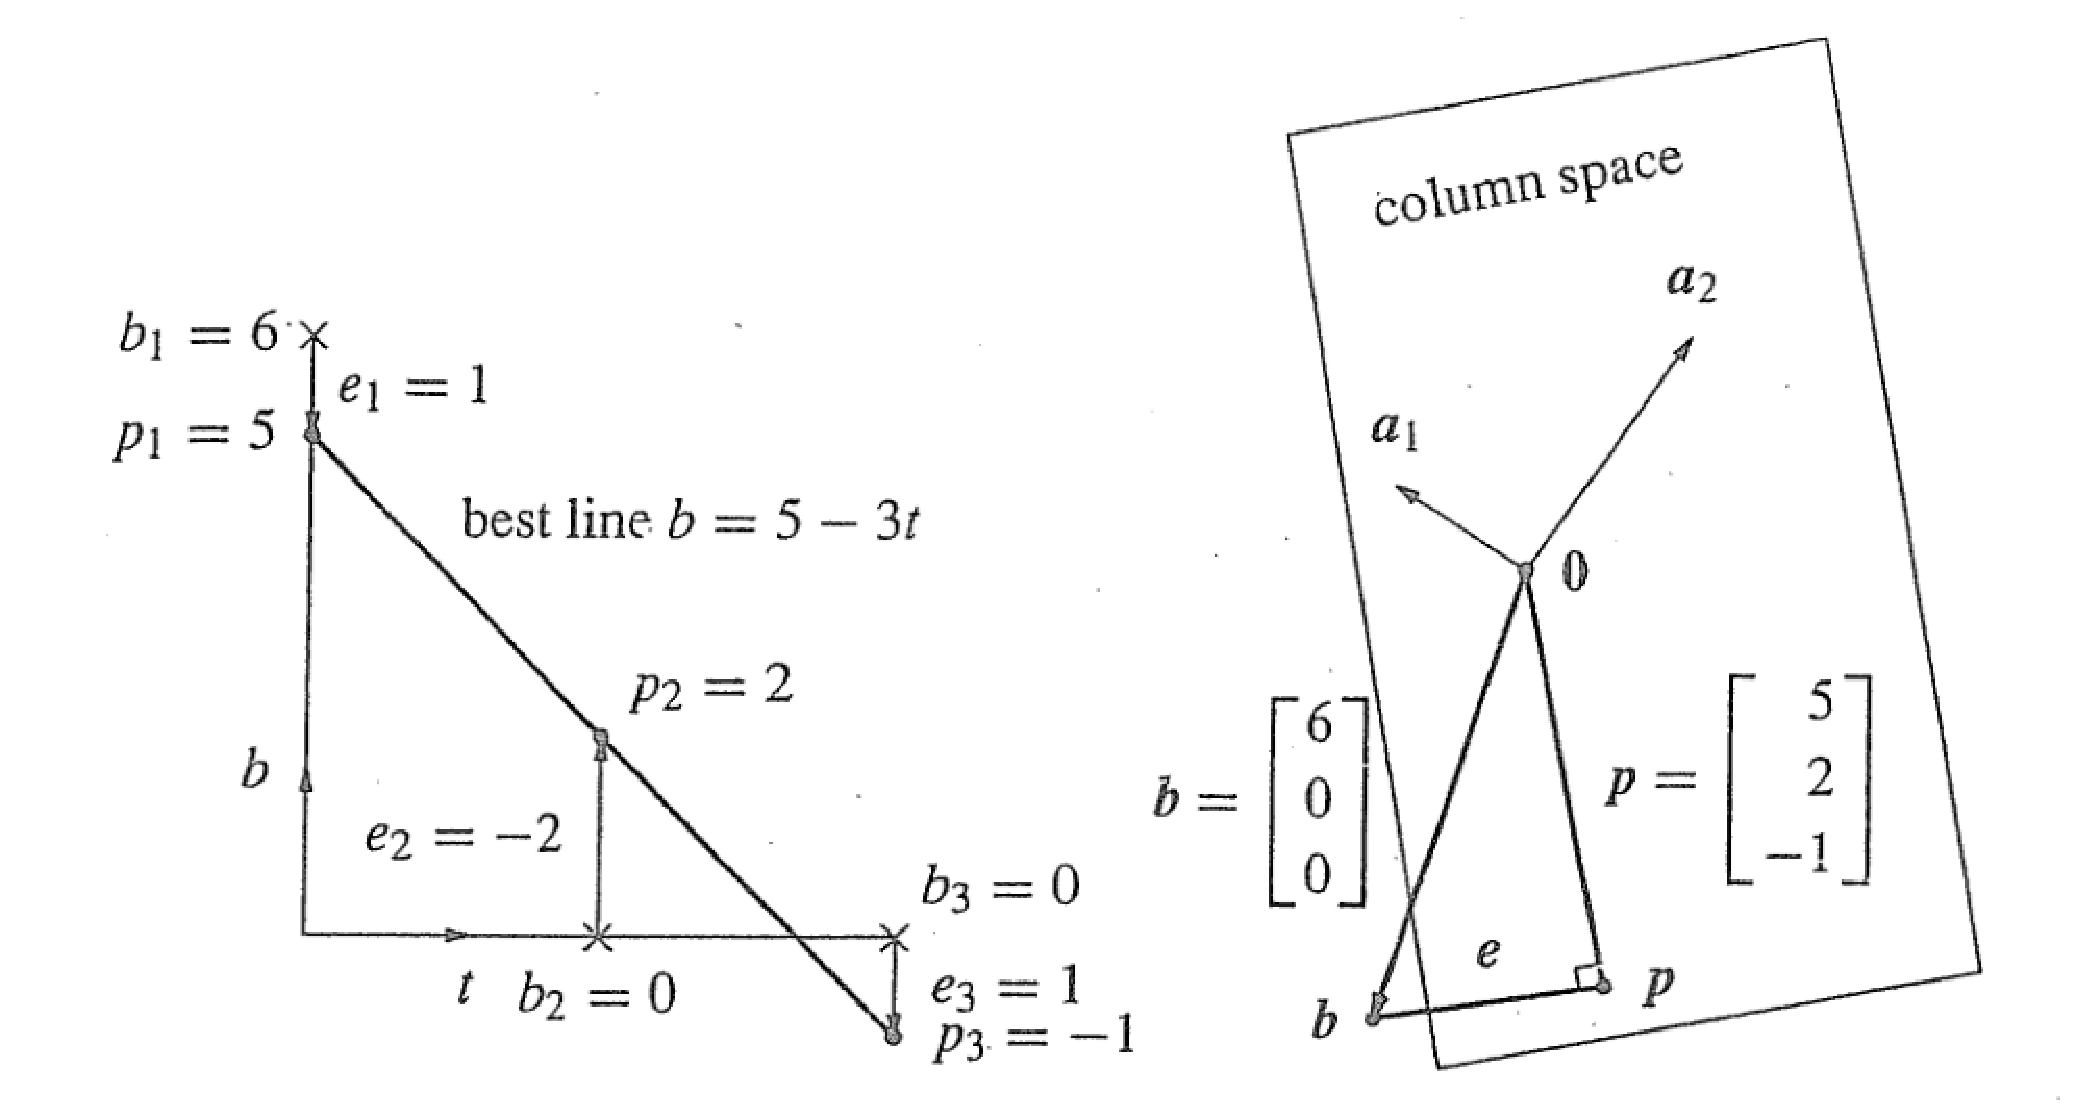
\includegraphics[width=0.7\linewidth]{TeX_files/Part02/chapter04/image/4-1}
	\caption[误差=到直线的垂直距离]{}
	\caption{}
	\label{fig:4-1}
\end{figure}

图4.1\;最好的线和投影:两张图片,同样的问题。这条线有顶点$p=(5,2,-1)$,误差$e=(1,-2,1)$。方程式$A^TA\hat{x}=A^Tb$给出结果$\hat{x}=(5,-3)$,最好的线为$5-3t$,第二张图片中,b的投影为$p=5a_1-3a_2$。

没有直线$b=C+Dt$通过这三个点。我们要求两个数C和D,满足三个方程,这是方程在$t = 0,1,2$匹配给定值$b= 6,0,0$:

	t=0   第一个点在直线$b=C+Dt$  则  $C+D*0=6$ 
	
	t=1   第二个点在直线$b=C+Dt$  则  $C+D*1=0$
	
	t=2   第三个点在直线$b=C+Dt$  则  $C+D*2=0$	
这个3×2的系统没有解决方案:$b =(6,0,0)$不是列(1,1,1)和(0,1,2)的组合。从这些方程中读取A,x和b,解答$A^TA\hat{x}=A^Tb$:

\begin{equation*}
  	A=              
\begin{bmatrix}
    1 & 0 \\ 1 & 1 \\ 1 & 2
\end{bmatrix}
  	\ x=
\begin{bmatrix}
	C \\ D
\end{bmatrix}
  	\ b=
\begin{bmatrix}
	6 \\ 0 \\0
\end{bmatrix}
\end{equation*}
$Ax=b$不可解。

	\subsection[最小化误差]{最小化误差\\Minimizing the Error}
	我们如何使误差$e=b-Ax$尽可能小呢?这是一个有着完美答案的问题。最佳x(被称之为$\hat{x}$)可以通过几何或代数或微积分找到:90°角,或投影向量b,或设置导数平方误差为零。
	
	根据几何学,每一个$Ax$都位于列(1,1,1)和(0,1,2)的平面,在那个平面(图\ref{fig:4-1})内,我们寻找最接近于b的点,最近点则是投影p。
	
	$A\hat{x}$的最佳选择是p,最小的可能错误为$e=b-p$。这三个点的高度$(p_1,p_2,p_3)$确实在一条直线上,因为p是系数C和D两列的组合。在拟合直线中,$\hat{x}$给出了最佳选择$(C,D)$。根据代数将每个向量B分成两部分。列空间中的部分是p,垂直部分在$A^T$零空间的误差为e。我们无法解答方程$(Ax=b)$,但是我们确实可以解答方程$A\hat{x}=p$(通过删除e):
	
	\begin{equation}
	Ax = b = p + e    A\hat{x} = p
	\end{equation}
	前者不可解,后者可解。
	$A\hat{x} = p$解法使得最小可能误差(也就是e),任何x的平方长度为:
	\begin{equation}
 	\|Ax-b\|^2 = \|Ax-p\|^2 + \|e\|^2
	\end{equation}
	
	这是直角三角形定律:$c^2=a^2+b^2$任何在列空间的向量$Ax-p$都垂直于e在$A^T$零空间的误差e,我们通过选择$x=\hat{x}$使$Ax-p$减小到零,让最小的可能误差为$e=(e_1,e_2,e_3)$。
	
	要注意“最小”的含义。$Ax-b$的平方长度最小化:最小二乘解法$\hat{x}$使得$E=\|Ax-b\|^2$尽可能小。
	
	图\ref{fig:4-1}左面板,展示了最接近的线,距离误差为$e_1,e_2,e_3 = 1,-2,1$,这些都是垂直距离,最小二乘线最小化为$E=e^2_1+e^2_2+e^2_3$。
	
	图\ref{fig:4-1}右面板,在三维空间(b,e,p空间)展示了相同的问题,向量b不在A的列空间中。这就是为什么我们无法解决$Ax=b$,没有直线通过这三个点,最小可能误差是垂直向量e,这是$e=b-A\hat{x}$,在三个方程中的误差向量(1,-2,1),与最好直线的距离。这两个数字的后面是基础方程$A^TA\hat{x}=A^Tb$。
	
	注意把误差1,-2,1加上0,误差$e=(e_1,e_2,e_3)$垂直于A的第一列(1,1,1),点乘得$e_1+e_2+e_3=0$。
	
	根据微积分,大多数函数最小化演算。图表最底部和各个方向导数都为零,这里的误差函数E最小平方和$e^2_1+e^2_2+e^2_3=0$(每个方程的误差平方):
	\begin{equation}
	E=\|Ax-b\|^2=(C+D\cdot 0-6)^2+(C+D\cdot 1)^2+(C+D\cdot 2)^2
	\end{equation}
	未知数为C和D,有两个未知数就有两个导数,最小值为零。它们是“偏导数”,因为$\partial E/\partial C$将D看做常数,$\partial E/\partial D$将C看做常数。
	\begin{equation*}
	\partial E/\partial C=2(C+D\cdot 0-6)+2(C+D\cdot 1)+2(C+D\cdot 2)=0
	\partial E/\partial D=2(C+D\cdot 0-6)(0)+2(C+D\cdot 1)(1)+2(C+D\cdot 2)(2)=0
	\end{equation*}
		
	$\partial E/\partial D$包含链式法则的额外因素$(0),(1),(2)$。(从$(C+2D)^2$的最后一个导数是2倍的$C+2D$的2倍),在C导数中对应的因素为1,1,1,因为C总是乘1,1,1,1和0,1,2是A的列并不是偶然的。
	
	现在取消所有项的2倍,收集所有的C和D:
	
	C和D的导数为0:
	\begin{equation}
	3C+3D=6 
	\quad 3C+5D=0 
	\quad A^TA=
	\begin{bmatrix}
	3 & 3 \\ 3 & 5
	\end{bmatrix}
	\end{equation}
	这些方程与$A^TA\hat{x}=A^Tb$是相同的,最好的C和D组成了$\hat{x}$。微积分的方程与线性代数的“正常方程”是相同的,这些是最小二乘的关键方程,当$A^TA\hat{x}=A^Tb$偏导数$\|Ax-b\|^2$为0。
	
	答案为$C=5,D=-3$,因此$b=5-3t$是最好的直线,它与三个点最为接近。当$t=0,1,2$时,这条直线经过$P=5,2,-1$,不能通过$b=6,0,0$,误差为$1,-2,1$,即为向量e。
	
	当x具有微小误差$\Delta x$时,$E=\|b-Ax\|$的一个微积分捷径零导数可以除去E中线性$\Delta x$项,我们可以直接计算线性项:
	\begin{equation*}
	(b-Ax-A\Delta x)^T(b-Ax-A\Delta x)
	\end{equation*}
	包含
	\begin{equation*}
	-\Delta x^TA^T(b-Ax)
	\end{equation*}
	
	相同的项也来自于$(b-Ax)^T(-A\Delta x)$。(记住真正的点产品有$y^Tz=z^Ty$)因此线性部分是这项的两倍,误差$\Delta x$的必须为零:$-\Delta x^TA^T(b-Ax)=0$要求$A^T(b-Ax)=0$。
	
	我们已经恢复在最小化$x=\hat{x}$正常方程$A^TA\hat{x}=A^Tb$。
	
	\subsection[统计与概率的线性代数]{统计与概率的线性代数\\Linear Algebra for Statistics and Probability}
	统计通常处理大量的数据,由于数据往往以矩阵形式存放,我们希望看到$A^TA$,最小二乘$Ax\approx b$是一个线性回归问题,最佳解$hat{x}$适合m个观测值和小于m的n个参数,这是线性代数在统计学中的一个基本应用。
	
	这一章节超越$A^TA\hat{x}=A^Tb$,这些未加权方程假设观测值$b_1,...,b_m$同样可靠,当有好的理由要求在一些观测值中有更高的精度(更小的方差)时,这些方程应该权更重,给予它们多大权重呢?$w_1,...,w_m$?如果观测值$b_i$不独立,协方差矩阵$\Sigma$给出统计误差,下面是关键问题:
	
	1、加权最小二乘和$A^TCA\hat{x}=A^TCb$。
	
	2、方差$\sigma^2_1,...,\sigma^2_m$和协方差矩阵$\Sigma=C^-1$。
	
	\subsection[加权最小二乘]{加权最小二乘\\Weighted Least Squares}
	为了在m个方程$Ax=b$中包含权重,每个方程i乘以权重$w_i$,将这m个权重放入对角矩阵,用$WAx=Wb$代替$Ax=b$,我们希望用最小二乘刚好解决这些方程。
	
	最小二乘方程由$A^TA\hat{x}=A^Tb$变为$(WA)^TWA\hat{x}=(WA)^TWb$。矩阵$C=W^TW$包含$(WA)^TWA$,在最小二乘的中间。
	
	加权最小二乘:
	\begin{equation}
	C=W^TW    A^TCA\hat{x}=A^TCb
	\end{equation}
	当n=1时,A的列数为1,$\hat{x}$从平均数变为加权平均数,最简单的例子:
	\begin{equation}
	\hat{x}=\frac{b_1+...+b_m}{m}
	\end{equation}
	改变为:
	\begin{equation*}
	\hat{x}_W=\frac{w^2_1b_1+...+w^2_mb_m}{w^2_1+...+w^2_m}
	\end{equation*}
	
	平均数$\hat{x}_W$给具有最大权重的观测值$b_i$最大的权重$w_i$,我们总是假设误差为零均值(如果必要的话减去平均数,在测量中并没有片面的偏见)。
	
	我们应该如何选择权重$w_i$?这取决于$b_i$的可靠性,如果观测值方差为$\sigma^2_i$,则$b_i$的均方根误差为$\sigma_i$。当我们以$\sigma_1,...,\sigma_m$分割方程时(左侧和右侧一起),所有的方差等于1。所以权重为$w_i=1/\sigma_i$,$C=W^TW$的对角线包含数字$1/\sigma^2_i$。
	
	统计正确矩阵为:$C=diag(1/\sigma^2_1,...,\sigma^2_m)$。
	
	这仅仅在假设不同方程的误差$e_i$和$e_j$独立时才正确(我们很快定义独立性,方差和协方差)。如果误差是相关的,非对角线元素将在协方差矩阵$\Sigma$中呈现,好的选择仍然是$C=\Sigma^-1$,将在以下章节中描述。
